% Source: research/oof-prioritization-2026-11-07/results.json; generated assets pin SHA256.
\subsubsection{Equal-Budget Retrospective Mutation Prioritisation}\label{sec:res-prioritization}
The 7 November follow-up applies the design in Section~\ref{sec:priority-methods} to the same
235-peptide W cohort. Candidate counts range from 216 to 532, so every peptide supplies ten
selections and every policy has the same total budget of \nPrioritySelections{}.
All 37 peptides without a positive hit remain in positive Precision@10; positive recall,
enrichment and budget-to-recall use 198 peptides in 190 groups. The negative endpoint retains
all 235 peptides for precision and uses 151 hit-containing peptides for recall.

\begin{table}[htbp]
  \centering
  \caption[Equal-budget replay on W]{Equal-budget replay on W. P and R are peptide-macro precision and recall in percent.
  Positive recall uses 198 peptides with hits; precision uses all 235. Each policy selects
  2,350 substitutions per endpoint. Random hits are analytic expectations.}
  \label{tab:priority-main}
  % Generated by build_prioritization_assets.py; retrospective development OOF.
% Source: research/oof-prioritization-2026-11-07/results.json
% SHA256: 4016cb5686f3520956cdc49268e2ea5363e678a6f1ce8555cec53e19a6938b87
{\small\setlength{\tabcolsep}{4pt}
\begin{tabularx}{\textwidth}{Xrrrr}
\toprule
Policy & P@10 (+) & Hits (+) & R@10 (+) & P@10 ($-$) \\
\midrule
LoRA-D & 53.62 & 1,260 & 16.62 & 14.00 \\
Ridge W5-D & 46.26 & 1,087 & 13.41 & 4.34 \\
Random expectation & 9.78 & 229.86 & 1.93 & 1.33 \\
Frozen-D & 47.83 & 1,124 & 13.71 & 10.17 \\
LoRA-B & 53.96 & 1,268 & 15.56 & 13.19 \\
\bottomrule
\end{tabularx}}

\end{table}

LoRA-D identifies \nPriorityLoraHits{} measured positive hits, versus \nPriorityWfiveHits{} for
W5-D and an expected \nPriorityRandomHits{} for random selection
(Table~\ref{tab:priority-main}). Its \nPriorityLoraPrecision\% precision is
\nPriorityDeltaWfive{} percentage points above W5-D and \nPriorityDeltaRandom{} above random.
Both adjusted intervals exclude zero (Table~\ref{tab:priority-contrasts}), supporting both
primary comparisons within this replay. LoRA-D yields \nPriorityExtraHits{} additional hits over
W5 under the same budget. These are known assay labels recovered by a retrospective selection
policy, not new experimentally confirmed predictions.

\begin{table}[htbp]
  \centering
  \caption[Primary positive Precision@10 differences, in percentage points]{Primary positive Precision@10 differences, in percentage points.
  Paired protein-group bootstrap uses 5,000 draws; 97.5\% intervals adjust the two primary contrasts.}
  \label{tab:priority-contrasts}
  % Generated by build_prioritization_assets.py; retrospective development OOF.
% Source: research/oof-prioritization-2026-11-07/results.json
% SHA256: 4016cb5686f3520956cdc49268e2ea5363e678a6f1ce8555cec53e19a6938b87
{\small\setlength{\tabcolsep}{4pt}
\begin{tabularx}{\textwidth}{Xrrr}
\toprule
LoRA-D minus & Difference (pp) & 95\% CI & 97.5\% CI \\
\midrule
Ridge W5-D & +7.36 & $[3.88, 10.88]$ & $[3.36, 11.39]$ \\
Random expectation & +43.84 & $[39.16, 48.24]$ & $[38.64, 48.83]$ \\
\bottomrule
\end{tabularx}}

\end{table}

The controls qualify the interpretation. Frozen-D reaches 47.83\% positive precision, and the
descriptive LoRA-D-minus-Frozen-D difference is $+5.79$ percentage points with 95\% interval
$[2.76,8.90]$. LoRA-B reaches 53.96\%, slightly above D, but D-minus-B has interval
$[-2.06,1.34]$ percentage points and remains unresolved. The primary recipe is not changed after
seeing this secondary result. All three individual LoRA-D seeds exceed W5-D in point estimate,
but they share the same outer partition (Table~\ref{tab:priority-seeds}).

\paragraph{Recall and the required number of selections.}
Positive Recall@10 is \nPriorityLoraRecall\% for LoRA-D, compared with 13.41\% for W5-D and
1.93\% for random. Recall is averaged over the 198 hit-containing peptides, so it is not the
ratio of pooled selected hits to pooled hits. The budget needed to reach a known fraction of
each peptide's hits is reported separately in Table~\ref{tab:priority-recall-budget}.
Figure~\ref{fig:priority-budget} shows the positive-hit budget curves.
LoRA-D minus W5-D requires 10.67 fewer selections on average for 50\% recall, with descriptive
95\% interval $[-16.48,-4.96]$; the 80\% difference is $-16.17$, interval $[-24.45,-7.64]$.
These are replay selection differences. Total hit counts would be unknown in a new assay,
and substitutions need not have equal experimental costs.

\begin{table}[htbp]
  \centering
  \caption[Mean selections to reach a known positive-hit recall, on 198 peptides with hits]{Mean selections to reach a known positive-hit recall, on 198 peptides with hits.
  Each peptide target is rounded upward. Random values are expected order-statistic ranks.}
  \label{tab:priority-recall-budget}
  % Generated by build_prioritization_assets.py; retrospective development OOF.
% Source: research/oof-prioritization-2026-11-07/results.json
% SHA256: 4016cb5686f3520956cdc49268e2ea5363e678a6f1ce8555cec53e19a6938b87
{\small\setlength{\tabcolsep}{4pt}
\begin{tabularx}{\textwidth}{Xrr}
\toprule
Policy & 50\% hit recall & 80\% hit recall \\
\midrule
LoRA-D & 71.32 & 154.36 \\
Ridge W5-D & 81.99 & 170.53 \\
Random expectation & 255.51 & 404.48 \\
\bottomrule
\end{tabularx}}

\end{table}

\begin{figure}[htbp]
  \centering
  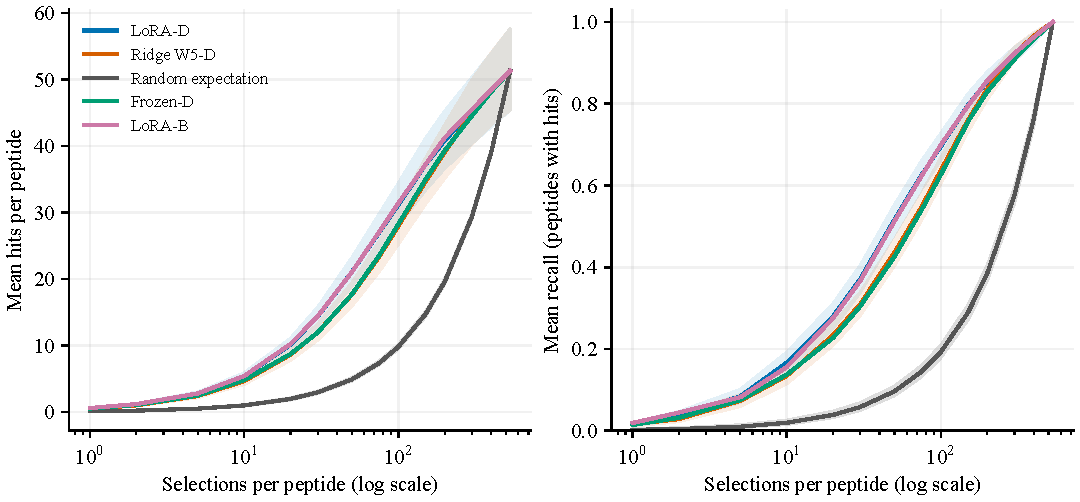
\includegraphics[width=\textwidth]{assets/ch4/fig-priority-budget.pdf}
  \caption[Positive-hit budget curves from the stored OOF replay]{Positive-hit budget curves from the stored OOF replay. Budgets are capped by available
  candidates; the horizontal axis is logarithmic. Coloured bands show 95\% group-bootstrap
  intervals for each LoRA-D or W5-D curve, not their difference. The grey band shows 95\%
  conditional random-allocation variation from 2,000 permutations, distinct from group uncertainty.}
  \label{fig:priority-budget}
\end{figure}

\paragraph{Other budgets, negative effects and WT-PSI strata.}
LoRA-D positive precision is 54.89\% at five selections and 50.55\% at twenty, compared with
47.91\% and 43.04\% for W5-D. Fractional budgets have different total selection counts and
must not be read as fixed ten-mutation budgets (Table~\ref{tab:priority-budgets}).
At the negative endpoint, LoRA-D precision is \nPriorityLoraNegativePrecision\%, with 329 hits,
versus 4.34\% and 102 hits for W5-D; random has expected precision 1.33\% and 31.16 hits.
The negative LoRA-D-minus-W5 difference is $+9.66$ percentage points, descriptive 95\% interval
$[7.13,12.35]$. Positive and negative directions are reported separately.

\begin{table}[htbp]
  \centering
  \caption[Positive Precision@10 by WT-PSI stratum, in percent]{Positive Precision@10 by WT-PSI stratum, in percent. Peptides without positive hits
  remain in precision; zero-event strata do not supply recall or enrichment evidence.}
  \label{tab:priority-strata}
  % Generated by build_prioritization_assets.py; retrospective development OOF.
% Source: research/oof-prioritization-2026-11-07/results.json
% SHA256: 4016cb5686f3520956cdc49268e2ea5363e678a6f1ce8555cec53e19a6938b87
{\small\setlength{\tabcolsep}{4pt}
\begin{tabularx}{\textwidth}{Xrrrr}
\toprule
WT PSI & Peptides & No (+) hit & LoRA-D P@10 & W5-D P@10 \\
\midrule
$\le3$ & 91 & 0 & 71.10 & 62.64 \\
$(3,4]$ & 85 & 2 & 63.76 & 52.59 \\
$(4,5]$ & 36 & 12 & 19.72 & 19.44 \\
$>5$ & 23 & 23 & 0.00 & 0.00 \\
\bottomrule
\end{tabularx}}

\end{table}

The positive gain is not uniform: the $(4,5]$ stratum has point precisions 19.72\% and 19.44\%,
whereas all 23 peptides above WT PSI 5 have no positive hit (Table~\ref{tab:priority-strata}).
Observed fold-level positive differences favour LoRA-D, but fold/seed summaries are not
independent studies. No exact score tie crosses any evaluated budget cutoff, including all
100 tie-seed sensitivity orders. The existing top-fraction helper and the hash-tie implementation
therefore give the same precisions on the checked data; this is numerical agreement, not an
independent benchmark.

\paragraph{What the replay adds.}
The result supplies a direct, same-candidate, same-budget comparison with both random and a
trained Ridge baseline. Independent arithmetic reconstruction matches all 14,100 ensemble
peptide--policy--endpoint--budget rows and the two primary intervals. It does not add a new
biological sample. The analysis takes about 102 seconds with 1.06~GiB peak process resident set
size on Linux under Windows Subsystem for Linux; these are scoring resources only. The development cohort has
informed previous choices, and cross-runtime LoRA--Ridge differences do not isolate adaptation.
Prospective wet-lab validation, actual time/cost savings and external generalisation remain open.
